%%
%% This is file `sample-manuscript.tex',
%% generated with the docstrip utility.
%%
%% The original source files were:
%%
%% samples.dtx  (with options: `all,proceedings,bibtex,manuscript')
%% 
%% IMPORTANT NOTICE:
%% 
%% For the copyright see the source file.
%% 
%% Any modified versions of this file must be renamed
%% with new filenames distinct from sample-manuscript.tex.
%% 
%% For distribution of the original source see the terms
%% for copying and modification in the file samples.dtx.
%% 
%% This generated file may be distributed as long as the
%% original source files, as listed above, are part of the
%% same distribution. (The sources need not necessarily be
%% in the same archive or directory.)
%%
%%
%% Commands for TeXCount
%TC:macro \cite [option:text,text]
%TC:macro \citep [option:text,text]
%TC:macro \citet [option:text,text]
%TC:envir table 0 1
%TC:envir table* 0 1
%TC:envir tabular [ignore] word
%TC:envir displaymath 0 word
%TC:envir math 0 word
%TC:envir comment 0 0
%%
%% The first command in your LaTeX source must be the \documentclass
%% command.
%%yes l

\documentclass[manuscript,screen]{acmart}

\usepackage{graphicx} % Required for \resizebox, \includegraphics
\usepackage{standalone} % Required for \includestandalone
\usepackage{tikz} % Load tikz
\usepackage{pgfplots} % Load pgfplots
\pgfplotsset{compat=newest} % Use the newest version for features
\usepgfplotslibrary{statistics} % Add this for potentially needed plot functions
\usetikzlibrary{
    shapes.geometric, % For shapes like diamond, trapezium, cylinder
    arrows.meta,      % For arrow tip styles
    positioning,      % For relative positioning (below=of ...)
    fit,              % To fit nodes around others
    backgrounds,      % To draw behind nodes
    shadows           % For subtle shadows
}

%%
%% \BibTeX command to typeset BibTeX logo in the docs
\AtBeginDocument{%
  \providecommand\BibTeX{{%
    Bib\TeX}}}

%% Rights management information.  This information is sent to you
%% when you complete the rights form.  These commands have SAMPLE
%% values in them; it is your responsibility as an author to replace
%% the commands and values with those provided to you when you
%% complete the rights form.
\setcopyright{acmlicensed}
\copyrightyear{2025}
\acmYear{2025}

%%
%% For managing citations, it is recommended to use bibliography
%% files in BibTeX format.
%%
%% You can then either use BibTeX with the ACM-Reference-Format style,
%% or BibLaTeX with the acmnumeric or acmauthoryear sytles, that include
%% support for advanced citation of software artefact from the
%% biblatex-software package, also separately available on CTAN.
%%
%% Look at the sample-*-biblatex.tex files for templates showcasing
%% the biblatex styles.
%%

%%
%% The majority of ACM publications use numbered citations and
%% references.  The command \citestyle{authoryear} switches to the
%% "author year" style.
%%
%% If you are preparing content for an event
%% sponsored by ACM SIGGRAPH, you must use the "author year" style of
%% citations and references.
%% Uncommenting
%% the next command will enable that style.
%%\citestyle{acmauthoryear}

%%
%% end of the preamble, start of the body of the document source.
\begin{document}

%%
%% The "title" command has an optional parameter,
%% allowing the author to define a "short title" to be used in page headers.
\title{A Spatially-Aware Search Engine for Textual Content in Images}

%%
%% The "author" command and its associated commands are used to define
%% the authors and their affiliations.
\author{Pranav Ramesh}
\email{pranavramesh@college.harvard.edu}
\affiliation{%
    \institution{Harvard University}
    \city{Cambridge}
    \state{MA}
    \country{USA}
}

\author{Mohamed Zidan Cassim}
\email{mzcassim@college.harvard.edu}
\affiliation{%
    \institution{Harvard University}
    \city{Cambridge}
    \state{MA}
    \country{USA}
}

\author{Giovanni D'Antonio}
\email{giovannidantonio@college.harvard.edu}
\affiliation{%
    \institution{Harvard University}
    \city{Cambridge}
    \state{MA}
    \country{USA}
}

%%
%% By default, the full list of authors will be used in the page
%% headers. Often, this list is too long, and will overlap
%% other information printed in the page headers. This command allows
%% the author to define a more concise list
%% of authors' names for this purpose.
\renewcommand{\shortauthors}{Ramesh et al.}

%%
%% The abstract is a short summary of the work to be presented in the
%% article.
\begin{abstract}
    Standard image search engines often treat text within images as secondary metadata or ignore its spatial location. This limits users' ability to find images based on text appearing in specific visual areas. We present a spatially-aware textual image search engine designed to address this limitation. Our approach utilizes an inverted index mapping text n-grams to their normalized bounding box coordinates within images. Queries consist of text and an optional spatial region. Relevance scoring combines spatial factors (Intersection over Union and proximity) with n-gram length, weighted according to configurable parameters. To facilitate development and evaluation, we developed a pipeline for generating synthetic datasets with controlled text placement and ground truth. We evaluated our system against non-spatial baselines (keyword-only and n-gram-only) using Mean Average Precision (MAP) and Precision@k (P@k) on this synthetic data. Results demonstrate statistically significant improvements in ranking quality for both n-gram usage over keywords (MAP 0.21 vs 0.03) and spatial awareness over n-grams alone (MAP 0.67 vs 0.21), validating the effectiveness of incorporating both n-grams and spatial context. A visualization tool was also developed to aid in understanding search results.
\end{abstract}

%%
%% The code below is generated by the tool at http://dl.acm.org/ccs.cfm.
%% Please copy and paste the code instead of the example below.
%%
\ccsdesc[500]{Information systems~Information retrieval}
\ccsdesc[500]{Information systems~Retrieval tasks and goals~Image search}
\ccsdesc[300]{Computing methodologies~Computer vision~Object detection}
\ccsdesc[300]{Information systems~Indexing}
\ccsdesc[100]{Computing methodologies~Document analysis and representation~Optical Character Recognition (OCR)}
\ccsdesc[100]{Computing methodologies~Image processing}
\ccsdesc[100]{Information systems~Search engine architectures and scalability}

%%
%% Keywords. The author(s) should pick words that accurately describe
%% the work being presented. Separate the keywords with commas.
\keywords{image search, text localization, spatial search, n-grams, OCR, information retrieval}

\received{20 April 2025}
\received[revised]{12 May 2025}
\received[accepted]{5 June 2025}

%%
%% This command processes the author and affiliation and title
%% information and builds the first part of the formatted document.
\maketitle

\section{Introduction}

\subsection{Problem Statement}

Images frequently contain rich textual information, such as signs, labels, headlines, logos, or embedded text in documents and screenshots. Traditional image search systems primarily focus on visual features or global textual tags, often failing to leverage the specific content and location of text within the image. Users cannot easily query for images containing specific text within a particular visual region (e.g., "find photos with 'SALE' in the top-right corner" or "show screenshots where 'error message' appears near the bottom"). This lack of spatial awareness limits the precision and utility of text-based image retrieval.

\subsection{Motivation}

The ability to search for text within specific spatial regions of images unlocks numerous applications across multiple domains. Document analysis benefits by enabling users to find specific sections or figures in scanned documents based on headings or captions in known layout areas. In retail and e-commerce, such technology facilitates locating product images where price or discount tags appear in particular locations relative to the product. Scene understanding applications can identify street signs, shop names, or specific labels within photographs of complex scenes with greater accuracy when spatial relationships are considered. UI/UX researchers can leverage spatial text search to analyze screenshots and find instances where specific labels or error messages appear in certain interface elements. Additionally, accessibility is enhanced by enabling visually impaired users to query not just what text appears in an image, but where it is located.

To illustrate the practical utility more concretely, consider a case study in \textbf{Automated Data Entry from Scanned Documents}. Imagine processing a high volume of scanned invoices or receipts for accounting. While Optical Character Recognition (OCR) can extract all text from an image, accurately identifying the \textit{semantic role} of specific text snippets (e.g., distinguishing the "Total Amount" from line item prices, or the "Invoice Date" from a "Payment Due Date") is a significant challenge due to the wide variety of document layouts. A traditional keyword search for terms like "Total" or for date patterns might yield multiple ambiguous candidates scattered across the document.

This is where spatially-aware search offers a distinct advantage. By leveraging common layout conventions, the system can target queries to specific regions. For example, a query searching for text matching a monetary amount pattern (e.g., \verb|\$\d+\.\d{2}|) \textit{specifically within the normalized coordinates corresponding to the bottom-right quadrant} of the document is highly likely to isolate the final \textbf{Total Amount}. Similarly, querying for date-like text primarily within the \textit{top-right quadrant} can reliably extract the \textbf{Invoice Date}. This targeted spatial querying drastically reduces ambiguity compared to context-agnostic text search, significantly simplifying the development of robust automated data entry pipelines without requiring complex template matching or sophisticated layout analysis models for every document variant. It demonstrates how spatial awareness can act as a powerful heuristic for semantic disambiguation in structured documents.

Existing methods often rely on whole-image tags or complex scene understanding models that may not precisely capture localized text queries. A dedicated system focusing on spatial text search promises higher precision and user control for these tasks.

\subsection{Proposed Solution \& Contributions}

To address the limitations of traditional methods, we propose and implement \textbf{SATIAS (Spatially-Aware Textual Image Search)}, a search engine designed to retrieve images based not only on \textit{what} text they contain but also \textit{where} that text is located. The overall system pipeline involves an initial pre-processing step where an Optical Character Recognition (OCR) engine, such as Pytesseract \cite{Smith2007AnOV}, is employed to extract textual content and corresponding bounding boxes from input images. This structured metadata then serves as input to the core SATIAS components. The central idea is to move beyond simple keyword matching by creating an index that explicitly links textual content (represented as n-grams, typically sequences of 1 to 3 words) to its precise spatial location within each image. This is achieved by building an inverted index where keys are text n-grams and values are lists of occurrences, each storing the \texttt{image\_id} and the n-gram's \textbf{normalized bounding box} coordinates (percentages of image width/height) to ensure scale and aspect-ratio invariance. User queries can specify both a \texttt{query\_text}, which is parsed into n-grams, and an optional target \textbf{spatial region}, also represented as a normalized bounding box. Candidate images containing matching n-grams are retrieved via the index, and each potential match is evaluated using a novel, configurable scoring mechanism. This scoring combines \textbf{spatial relevance}—calculated as a weighted sum of \textbf{Intersection over Union (IoU)} for overlap and \textbf{centroid proximity} for nearness between the query region and the n-gram box—with \textbf{textual relevance}, where matches involving longer n-grams contribute more significantly. The relative importance of IoU versus proximity can be tuned via configuration weights. Finally, scores are aggregated per image, and the results are ranked to provide the user with images where the desired text appears in the specified location.

This paper details the design, implementation, and rigorous evaluation of the SATIAS system. Our primary contributions include: (1) the \textbf{novel algorithm design} itself, particularly the use of normalized coordinates for indexing and the hybrid spatial scoring function combining weighted IoU and proximity; (2) a robust and parallelized \textbf{synthetic data generation pipeline} (described in Section~\ref{sec:synthetic_data}) that creates large datasets with precise ground-truth bounding boxes and targeted queries, crucial for controlled offline evaluation independent of OCR errors; (3) a modular Python \textbf{system implementation} encompassing indexing, flexible query parsing, spatial calculations, and search logic; (4) a \textbf{rigorous quantitative evaluation} framework (using a dedicated script, see Section~\ref{sec:evaluation}) using MAP@k and P@k metrics to compare SATIAS against keyword-only and n-gram-only baselines on the synthetic data, including statistical significance testing (Wilcoxon signed-rank test); and (5) an \textbf{interactive visualization tool} (provided as an interactive script) with a GUI that allows users to execute searches and inspect results with overlays showing query regions and color-coded n-gram bounding boxes based on IoU, aiding qualitative analysis and debugging.

\begin{figure}[ht]
    \centering
    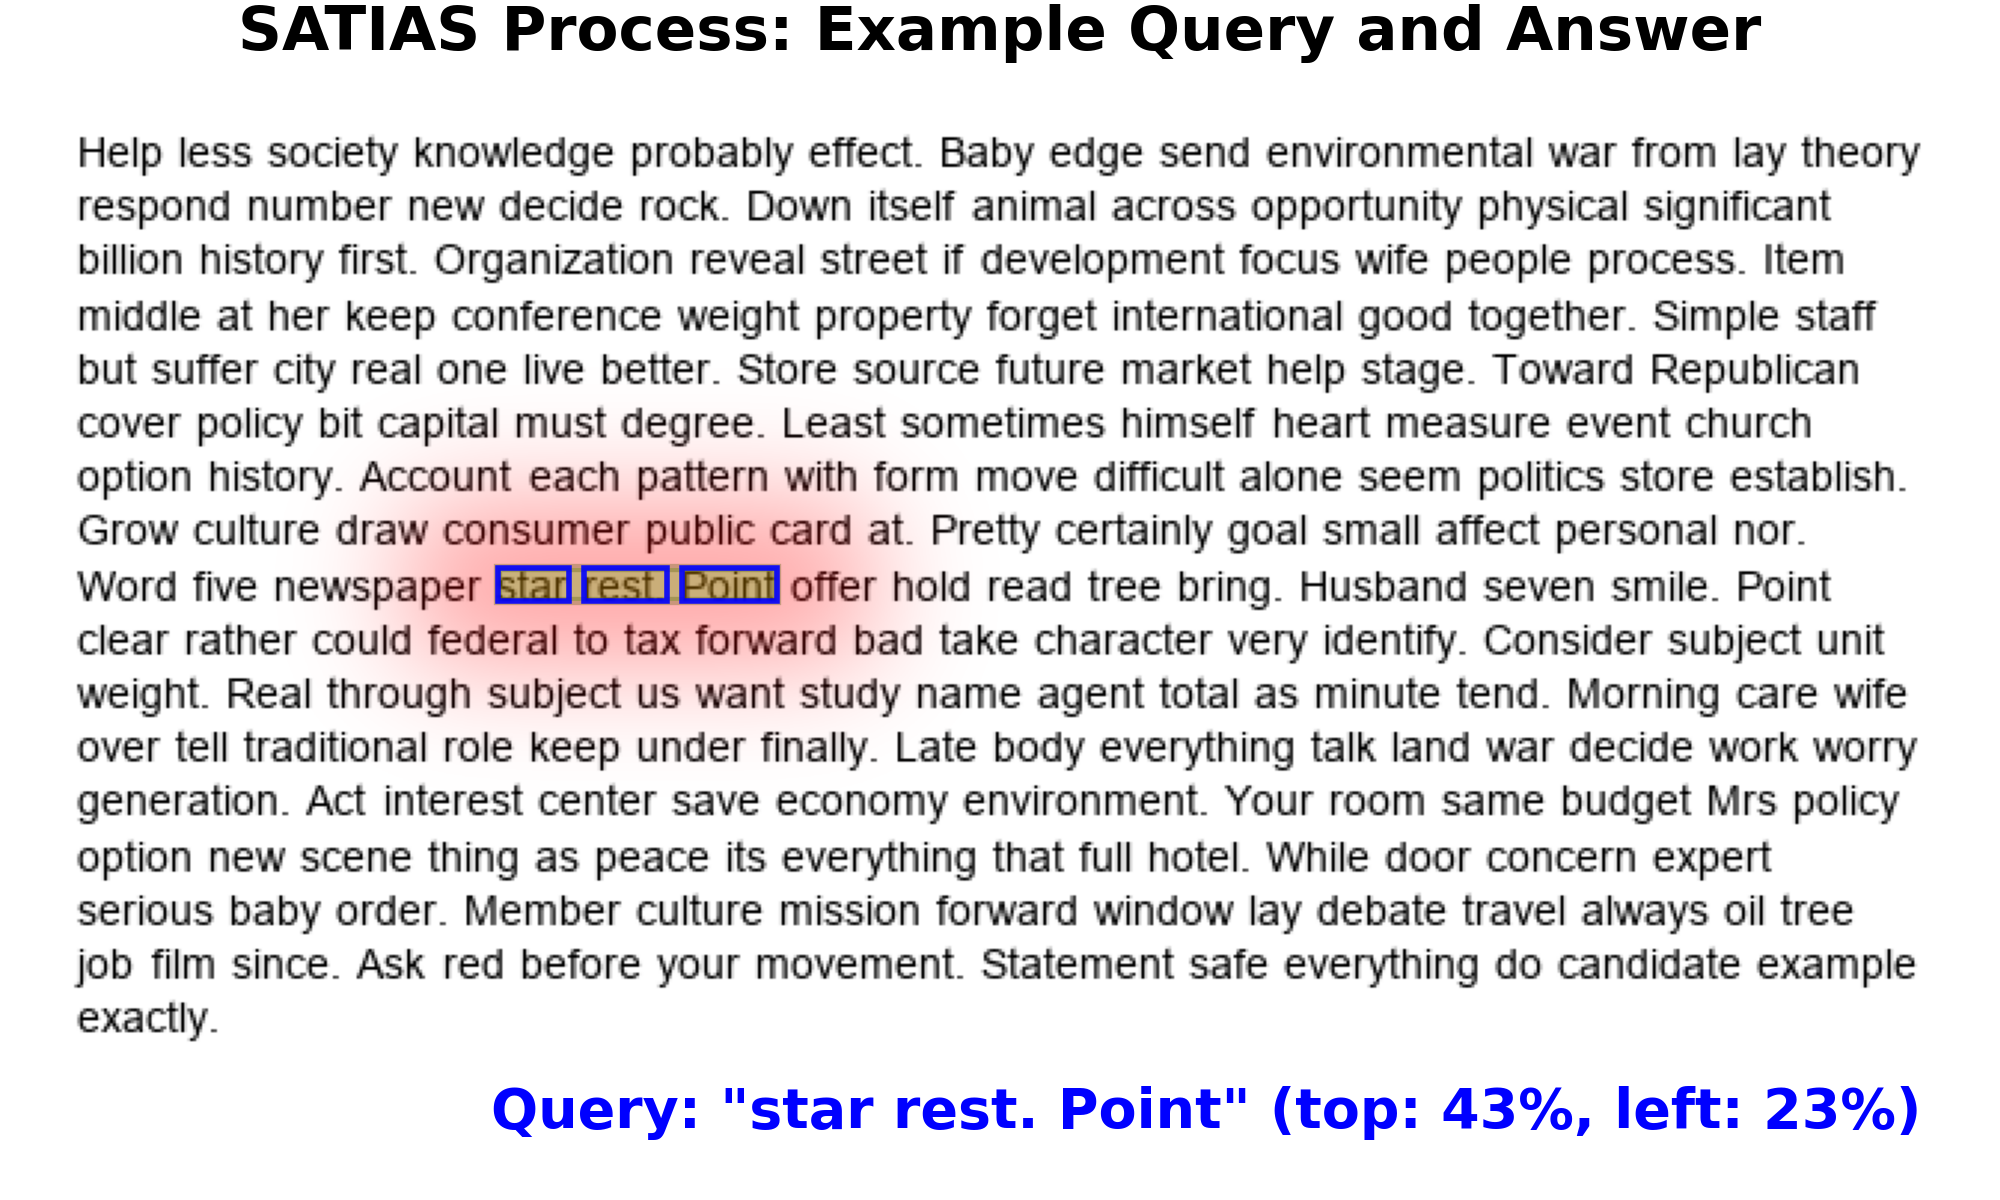
\includegraphics[width=0.95\linewidth]{satias_example.png}
    \caption{Illustration of the SATIAS process. The blue boxes indicate the n-gram query region, the heat overlay shows the answer area, and the query text at bottom right demonstrates a location-aware search.}
    \label{fig:satias-process}
\end{figure}

\section{Prior Work}
\label{sec:prior_work}

The challenge of searching for textual content within images, potentially constrained by location, has been explored from various perspectives. Our work draws upon foundational concepts while offering a specific, geometrically focused solution.

\subsection{Foundational and Explicit Spatial Methods}

\textbf{Region-Based Visual Similarity Search:} Foundational work in image retrieval explored various modalities. For instance, Manmatha et al. (UMass CIIR, 2000) \cite{Manmatha00} proposed a system focused on retrieving images based on \textbf{visual appearance similarity}. In their approach, users define salient regions of interest (e.g., parts of a car) on a query image, and the system uses filtered templates derived from these regions to find visually similar images in a database, effectively matching appearance across scale changes without requiring explicit segmentation. While this represents important early work in region-based querying, its focus is on visual features (shape, appearance) within those regions. This contrasts with our SATIAS system, which does not analyze visual appearance but instead focuses specifically on retrieving images where particular \textbf{textual content (n-grams)} is found within user-specified geometric \textbf{regions (bounding boxes)}, leveraging location as a key filter for text rather than matching visual similarity.

\textbf{Spatial-Semantic Approaches:} More recent work has integrated spatial reasoning with semantic understanding. Mai et al. (CVPR 2017) \cite{Mai17} proposed a spatial-semantic image search framework where users define semantic layouts on a canvas, and a Convolutional Neural Network (CNN) synthesizes corresponding visual features for retrieval. This differs from our approach, which focuses narrowly on matching the precise geometric location (bounding box) of specific text n-grams provided in the query, rather than interpreting broader semantic layouts.

\subsection{The Rise of MLLMs in Spatial Grounding}

Recent years have seen a significant shift towards utilizing Multimodal Large Language Models (MLLMs) for tasks involving spatial grounding. These models, such as KOSMOS-2 \cite{Huang24} and Groma \cite{Yin24}, aim to integrate visual perception, language comprehension, and spatial reasoning within unified architectures \cite{Wang23UniIR}, often trained on web-scale datasets \cite{Huang24}.

\textbf{Approach:} Instead of explicit geometric indexing and scoring like our system, MLLMs typically handle spatial information implicitly through learned mechanisms. These mechanisms include using location tokens where continuous bounding box coordinates are discretized into special tokens integrated into the language model's vocabulary \cite{Huang24}, leveraging cross-modal attention mechanisms to learn correlations between text and image regions \cite{Tan23ESA}, and utilizing joint embedding spaces that align visual regions and textual descriptions \cite{Karpathy15}, implicitly encoding spatial relationships.

\textbf{Comparison to Our System:} Compared to our system, MLLMs offer distinct advantages and disadvantages. MLLMs possess strong semantic understanding derived from their underlying LLMs, enabling them to handle synonyms, paraphrasing, and complex natural language queries describing spatial relations (e.g., "the book to the left of the lamp") \cite{Huang24, Yin24}, a capability our exact n-gram matching system lacks. However, the reasoning process of MLLMs is often opaque ("black box"), whereas our system, using explicit IoU and proximity calculations, offers greater interpretability and direct control via tunable weights. Additionally, training state-of-the-art MLLMs for grounding requires massive datasets (like the GRIT dataset used for KOSMOS-2 \cite{Huang24}) and significant computational resources for pre-training and fine-tuning \cite{Yin24}. Additionally, the data requirements for SATIAS differ: while it relies on an upstream OCR process, its core indexing logic utilizes the resulting text/bounding box data directly from images, unlike MLLMs that typically necessitate extensive pre-training on datasets with explicitly grounded text-region pairs. This trend towards MLLMs highlights a different paradigm for spatial understanding, trading explicit geometric control for learned semantic richness and query flexibility, albeit with associated challenges in interpretability and data requirements.

\subsection{Enabling Technologies}

\textbf{Text Spotting:} Accurate detection and bounding box generation are critical prerequisites for any text-in-image search system. The field has advanced to handle arbitrary text shapes using segmentation, contour embedding, Bezier curves (ABCNet), Mask R-CNN, or sequential deformation. However, bounding box inaccuracy remains a challenge for real-world geometric scoring.

\textbf{Indexing:} Scalability requires efficient indexing structures. While our approach uses an in-memory inverted index, spatial databases traditionally use R-Trees/Quadtrees, often combined with inverted indexes in hybrid structures. Recent Learned Sparse Retrieval (LSR) methods (e.g., STAIR \cite{Chen23}, Cao et al. \cite{Cao23}, Bai et al. \cite{Bai24}) map dense embeddings to sparse lexical vectors compatible with inverted indexes, offering a promising direction for scalable multimodal retrieval.

\subsection{Contributions}

Our work occupies a niche focused on precise, spatially constrained retrieval of specific text n-grams. Compared to the prior work, our contributions are:

\begin{enumerate}
    \item The use of an efficient inverted index mapping n-grams directly to normalized bounding boxes
    \item A tunable spatial scoring function explicitly combining geometric overlap (IoU) and centroid proximity, offering direct control over spatial relevance criteria
    \item A dedicated synthetic data generation pipeline and evaluation methodology designed to rigorously assess the performance of spatial text localization, isolating it from OCR errors and providing targeted spatial query scenarios
\end{enumerate}

Our approach provides a simple, interpretable method for precise geometric localization of exact text n-grams within rectangular regions. Its strengths are direct geometric control and the synthetic data pipeline for evaluation. Key limitations include dependence on OCR accuracy, lack of semantic understanding (unlike Visual-Semantic Embedding or attention models), limited query expressiveness (compared to canvas-based, trace-based, or relational queries), and scalability issues which can be addressed by spatial, hybrid, or Learned Sparse Retrieval (LSR) indexing techniques. It represents a valuable baseline but stands apart from dominant deep learning trends emphasizing semantics and learned alignments.

\subsection{Comparison of Approaches}

Table~\ref{tab:approaches} provides a comprehensive comparison of various spatially-aware image-text retrieval approaches, highlighting the distinctive positioning of our system among existing methods.

\begin{table*}
    \caption{Comparison of Spatially-Aware Image-Text Retrieval Approaches}
    \label{tab:approaches}
    \begin{tabular}{p{2.8cm}p{2.8cm}p{4.5cm}p{3.4cm}}
        \toprule
        Approach                                     & Query Type                & Key Characteristics                                                           & Strengths/Weaknesses                 \\
        \midrule
        Foundational Text-in-Image~\cite{Manmatha00} & Keywords                  & Text as document metadata; Inverted Index; Keyword matching                   & (+) Established base approach        \\
                                                     &                           &                                                                               & (-) No spatial awareness             \\
        \midrule
        Explicit Spatial-Semantic~\cite{Mai17}       & Text-boxes on canvas      & User-defined layout; Visual Feature Index; Feature similarity                 & (+) Flexible canvas input            \\
                                                     &                           &                                                                               & (-) Less precise text matching       \\
        \midrule
        VSE / Attention Models~\cite{Faghri17}       & Text Query                & Implicit spatial via embeddings; Learned attention mechanisms & (+) Strong semantic understanding    \\
                                                     &                           &                                                                               & (-) No explicit spatial queries      \\
        \midrule
        MLLMs (KOSMOS-2, Groma)                      & Natural Language          & Learned mechanisms; End-to-end approach                                       & (+) Semantic flexibility             \\
                                                     &                           &                                                                               & (-) Black-box reasoning              \\
        \midrule
        Our Approach                                 & N-grams + Optional Region & Normalized Bounding Boxes; Explicit IoU + proximity scoring                   & (+) Interpretable; Precise           \\
                                                     &                           &                                                                               & (-) Limited semantics; OCR dependent \\
        \bottomrule
    \end{tabular}
\end{table*}

\section{Methodology}

Our system comprises two main phases: offline indexing and online query processing/search.

\subsection{Core Algorithm Overview}

The system first preprocesses a collection of images (or uses pre-computed metadata in our synthetic case) to build an inverted index. This index maps text n-grams to a list of all locations (image ID and normalized bounding box) where they appear. During online search, a user query (text + optional region) is processed. N-grams are extracted from the query text. The inverted index is used to retrieve candidate image locations matching these n-grams. Each match is scored based on n-gram length and spatial relevance relative to the query region. Scores are aggregated per image, and results are ranked.

\subsection{Indexing Phase}

\paragraph{Objective} Create an efficient lookup structure for n-gram occurrences and their spatial locations.

\paragraph{Process} The indexer module consumes structured image metadata. In a typical real-world application, this metadata would be generated by running an upstream OCR engine (e.g., Pytesseract \cite{Smith2007AnOV}) on the input images to extract words and their bounding boxes. For the evaluations presented in this paper, however, the input metadata originates from our synthetic data generation pipeline (Section~\ref{sec:synthetic_data}), which provides perfect, programmatically determined ground-truth locations, bypassing the need for actual OCR during evaluation.

The core data structure employed is an inverted index mapping n-grams to their occurrences. Each key in this index is a text n-gram string, and the corresponding value is a list of occurrences, where each occurrence contains an image identifier and normalized bounding box coordinates. As the system processes each n-gram from the input data, it appends a new entry containing the image identifier and normalized bounding box to the list associated with that n-gram text. Once constructed, the entire index is serialized and saved to persistent storage, allowing efficient loading in subsequent search sessions without rebuilding the index.

\begin{figure*}[ht!] % Use figure* for spanning two columns if needed, [ht!] for placement preference
    \centering
    \includestandalone[width=0.95\textwidth]{satias_workflow_diagram} % Use includestandalone
    \caption{Overview of the SATIAS system workflow, detailing the offline indexing phase and the online search phase.}
    \label{fig:satias_workflow}
\end{figure*}

\subsection{Query Processing}

\paragraph{Objective} Convert user input into a format suitable for searching the index.

\paragraph{Process} The query processing stage transforms raw user input into structured data that can be efficiently matched against the inverted index. This process handles two key components: the query text and an optional spatial region specification. For the textual component, the system divides the input query text into individual words and generates all possible n-grams within the configured range (from the minimum to maximum n-gram length). This n-gram extraction mirrors the approach used during indexing, ensuring consistency between indexed content and query terms.

For the spatial component, the system parses an optional region string parameter, which can specify a target area within images using various formats (e.g., \verb|"top: 10-30, left: 50-70"|). This parsing interprets different notation styles for specifying top, left, bottom, and right boundaries or ranges as percentages of image dimensions. The parser performs validation on these values and handles edge cases gracefully. If the spatial region string is missing, invalid, or cannot be parsed, the system defaults to using the full image area represented as normalized coordinates \verb|[0.0, 0.0, 100.0, 100.0]|, effectively conducting a whole-image search. After processing both components, the function returns the complete query representation: a list of extracted query n-grams and a single normalized query bounding box ready for the search phase.

\subsection{Search and Ranking}

\paragraph{Objective} Retrieve and rank images based on textual and spatial relevance.

\paragraph{Process} The search process begins with the initialization of an image score accumulator, mapping each image ID to a score, initially zero. The overall score for an image $I$ given a query $Q = (Q_{text}, Q_{bbox})$ can be conceptually represented as:
\[
    \text{Score}(I, Q) = \sum_{q \in Q_{text}} \sum_{\text{occ} \in \text{Occ}(q, I)} \text{SpatialRel}(Q_{bbox}, \text{occ}_{bbox}) \times \text{Weight}(\text{len}(q))
\]
where $Q_{text}$ is the set of query n-grams, $\text{Occ}(q, I)$ are occurrences of n-gram $q$ in image $I$ with bounding box $\text{occ}_{bbox}$, $\text{SpatialRel}$ is the spatial relevance function, and $\text{Weight}$ depends on n-gram length.

For each query n-gram $q \in Q_{text}$, the system performs a lookup in the inverted index to retrieve all occurrences $\text{occ} \in \text{Occ}(q, I)$ across the indexed images (as shown in the online search phase of Figure~\ref{fig:satias_workflow}). When a query n-gram is found, the algorithm iterates through each occurrence, represented as a tuple of image identifier and normalized bounding box $\text{occ}_{bbox}$.

The scoring mechanism first determines the appropriate spatial relevance component, $\text{SpatialRel}(Q_{bbox}, \text{occ}_{bbox})$. For baseline non-spatial searches or when the query doesn't specify a region of interest (using the default full-image bounding box, $Q_{bbox}$), this component is set to 1.0, effectively ignoring spatial factors. However, when processing spatially-aware queries with specific target regions ($Q_{bbox}$), the system employs a sophisticated dual-metric approach. It calculates the Intersection over Union (IoU) between $Q_{bbox}$ and $\text{occ}_{bbox}$, which quantifies the degree of overlap. Simultaneously, it computes a proximity score based on the distance between centroids of $Q_{bbox}$ and $\text{occ}_{bbox}$, using an exponential decay function that rewards closer matches. These two metrics are then combined into a single spatial score using configurable weights (typically equal weights of 0.5 each): $\text{SpatialRel} = w_{iou} \times \text{IoU} + w_{prox} \times \text{Proximity}$. This hybrid approach effectively addresses the limitations of using either metric in isolation—IoU fails to reward nearby non-overlapping matches, while proximity alone would ignore the extent of overlap and relative sizes.

The algorithm then weights this spatial relevance by the n-gram length, $\text{Weight}(\text{len}(q))$, recognizing that longer matching phrases should contribute more significantly to relevance than shorter ones. This weighted score is added to the accumulated score for the corresponding image $I$. After processing all query n-grams and their occurrences, the system sorts the image scores in descending order and returns a ranked list of images with their relevance scores, representing the most relevant images for the given query.

This scoring approach provides a balance between textual and spatial relevance, with the configurable weights ($w_{iou}, w_{prox}$) offering flexibility to adjust the importance of exact overlap versus general proximity based on specific application needs. The n-gram length weighting further enhances discrimination, favoring images containing more specific, longer matching phrases over those with only short, potentially more ambiguous matches.

\subsection{Synthetic Dataset Generation}
\label{sec:synthetic_data}

\paragraph{Motivation} Generating a synthetic dataset provided several key advantages for our research. The approach allowed us precise control over text content, layout, and repetition within the images. We were able to obtain perfect pixel-level bounding boxes for every word and n-gram, effectively eliminating OCR errors as a confounding variable during algorithm development. This dataset generation also facilitated automatically creating queries with known ground truth target images and specific spatial relationships (overlap, proximity, etc.) to systematically test different scoring scenarios. Additionally, the synthetic approach offered scalability by efficiently generating large datasets (thousands of images, tens of thousands of queries) using parallel processing.

\paragraph{Process} The synthetic dataset generation process began with centralized configuration controlling parameters like image dimensions, number of images, font settings, text density, repetition control, word distinctiveness, n-gram range, and query generation. The core logic first created a pool of unique sentences to ensure controlled repetition of words and phrases across different images. For each image, we created a blank canvas and selected a random subset of sentences from the pool. We probabilistically injected specific test phrases (e.g., "special offer") multiple times at random locations within the selected text, and replaced some common words with more distinctive words to aid later visual inspection and analysis. Words were then drawn onto the image sequentially (top-down, left-right), handling line wrapping based on margins and word width, with text allowed to bleed off the bottom edge to ensure full vertical coverage. Crucially, we calculated the precise pixel bounding box \verb|[top, left, bottom, right]| for each individual word before drawing and stored this information.

After generating the words and their positions, we calculated all n-grams within the configured range (e.g., 1 to 3 words) for each image. For each n-gram, we determined the union bounding box (in pixels) based on the exact pixel bounding boxes of its constituent words. The query generation process then created a set number of queries for each image by selecting a random n-gram already placed in that image as the textual target, with its location serving as the ground truth. We randomly chose a query region type based on the configured distribution (e.g., No Region, Exact Match, High IoU, Low IoU, Nearby, Distant) and generated a corresponding normalized query region based on the target n-gram's location and the chosen type. To maximize efficiency, we parallelized the generation process across multiple CPU cores.

\paragraph{Output} The generation pipeline produced several essential outputs: the synthetic images themselves, comprehensive metadata containing details about each image and lists of all words and n-grams within it along with their exact pixel bounding boxes, and a queries dataset containing all generated queries. Each query record includes a query identifier, ground truth image identifier, query text, normalized target region coordinates, ground truth bounding boxes for the text, and information about how the query region was created relative to the target text. This structured output provided all necessary information for training and evaluating our spatial search algorithms.

This approach of programmatically determining text locations, rather than running an OCR engine on the generated images, provides perfect ground-truth bounding boxes. This allows the evaluation (Section~\ref{sec:evaluation}) to focus specifically on the performance of the SATIAS indexing and search algorithms, isolating it from potential inaccuracies or variations introduced by an external OCR process.

\section{Evaluation}
\label{sec:evaluation}

We conducted a quantitative evaluation to assess the performance of the spatially-aware search engine compared to relevant non-spatial baselines, using the generated synthetic dataset.

\subsection{Evaluation Setup}

The evaluation utilized a large synthetic dataset consisting of 50,000 queries derived from 2,000 generated images. For each query, we defined the single "relevant" image as the one specified in the query record—specifically, the image from which the query's target n-gram was originally sampled. All other images were considered non-relevant for that query. We compared SATIAS against two non-spatial baselines, as detailed below. All metrics were calculated using a cutoff of k=10.

\subsection{Evaluation Metrics}
\label{sec:evaluation_metrics}

To quantify the performance of our spatially-aware search system and compare it against the non-spatial baselines, we utilized standard information retrieval metrics calculated using the `evaluate.py` script on the generated `queries.json` dataset. Given the nature of our synthetic queries, where each query has exactly one known ground-truth relevant image, the primary metrics employed are:

\begin{itemize}
    \item \textbf{Mean Average Precision (MAP):} This is the mean of the Average Precision (AP) scores calculated for each query. Since each query has only a single relevant document in our setup, the AP for a single query simplifies to $1/\text{rank}$ if the correct image is found within the top $k$ results, and 0 otherwise. MAP provides an overall measure of ranking quality across the entire query set, considering the position of the relevant item.
    \item \textbf{Precision at k (P@k):} This is the average, across all queries, of the precision calculated at a cutoff rank $k$. Precision@k for a single query measures the proportion of relevant items among the top $k$ retrieved results. In our single-relevance case, P@k for one query is $1/k$ if the correct image is in the top $k$, and 0 otherwise. The mean P@k indicates, on average, how often the correct item appears within the top $k$ results.
\end{itemize}

We report both MAP and P@k for $k=1, 5, 10$, as implemented in our evaluation script. Furthermore, the individual Average Precision (AP) scores for each query were used as input for the Wilcoxon signed-rank test to determine the statistical significance of performance differences between the compared system configurations (SATIAS vs. N-gram Baseline, and N-gram Baseline vs. Keyword Baseline), as detailed in Section \ref{sec:results}.

\subsection{Baselines}
\label{sec:baselines}

To effectively evaluate the contribution of spatial awareness and n-gram usage, we compared SATIAS against two simpler baseline configurations:

\begin{itemize}
    \item \textbf{N-gram Baseline:} This configuration uses n-grams but operates non-spatially (`search\_mode="ngram\_text\_only"`). It ignores the query region and uses a fixed `spatial\_score\_component` of 1.0, effectively ranking based only on the presence and length of matching n-grams. This baseline helps isolate the performance impact of using n-grams compared to simple keywords, independent of spatial scoring.
    \item \textbf{Keyword Baseline:} This represents a rudimentary non-spatial search (`search\_mode="keyword\_only"`). It breaks the query text into unique words and scores images based simply on the count of matching words found anywhere in the image. This baseline ignores both n-grams and location information, serving as a fundamental comparison point.
\end{itemize}

Note that while other approaches like spatial-semantic search \cite{Mai17}, visual-semantic embeddings, and MLLMs \cite{Huang24, Yin24} were discussed in Section~\ref{sec:prior_work}, they are not included in this quantitative comparison. Spatial-semantic methods target visual layout matching, a different task from our precise text localization. VSE and attention models generally lack mechanisms for explicit geometric constraints, and benchmarking against MLLMs requires significant resources and query adaptation beyond the scope of this evaluation, which focuses on isolating the impact of our explicit geometric scoring against non-spatial text retrieval baselines.

\subsection{Results}
\label{sec:results}

The evaluation was conducted on a dataset containing 50,000 queries with a cutoff of k=10. Table~\ref{tab:results} summarizes the performance metrics for all three approaches.

\begin{table*}[t]
    \centering
    \caption{Performance Comparison of Search Methods (N=50,000 queries)}
    \label{tab:results}
    \begin{tabular}{lccc}
        \toprule
        \textbf{Metric} & \textbf{SATIAS} & \textbf{N-gram Baseline} & \textbf{Keyword Baseline} \\
        \midrule
        MAP             & 0.6711          & 0.2110                   & 0.0312                    \\
        \midrule % Added separator for clarity
        P@1 (Max: 1.0)  & 0.6006          & 0.1490                   & 0.0067                    \\
        P@5 (Max: 0.2)  & 0.1487          & 0.0459                   & 0.0061                    \\
        P@10 (Max: 0.1) & 0.0795          & 0.0324                   & 0.0058                    \\
        \bottomrule
    \end{tabular}
\end{table*}

\paragraph{Statistical Analysis}

To assess the significance of these results, we performed pairwise Wilcoxon signed-rank tests on the Average Precision (AP) scores for each query. The following p-values were obtained:

\begin{itemize}
    \item \textbf{SATIAS vs. N-gram Baseline:} p-value = 0.0000
    \item \textbf{N-gram Baseline vs. Keyword Baseline:} p-value = 0.0000
    \item \textbf{SATIAS vs. Keyword Baseline:} p-value = 0.0000
\end{itemize}

All p-values are less than 0.0001, indicating that the observed differences are highly statistically significant. The 95\% confidence intervals for MAP were [0.669, 0.673] for SATIAS, [0.209, 0.213] for N-gram Baseline, and [0.031, 0.032] for Keyword Baseline. For P@1, the 95\% confidence intervals were [0.599, 0.602] for SATIAS, [0.148, 0.150] for N-gram Baseline, and [0.0066, 0.0068] for Keyword Baseline. For P@5, the 95\% confidence intervals were [0.147, 0.150] for SATIAS, [0.045, 0.047] for N-gram Baseline, and [0.0059, 0.0063] for Keyword Baseline. For P@10, the 95\% confidence intervals were [0.078, 0.081] for SATIAS, [0.031, 0.033] for N-gram Baseline, and [0.0056, 0.0060] for Keyword Baseline.

Overall, SATIAS achieved a MAP of 0.6711 (95\% CI: [0.669, 0.673]), a P@1 of 0.6006 (95\% CI: [0.599, 0.602]), a P@5 of 0.1487 (95\% CI: [0.147, 0.150]), and a P@10 of 0.0795 (95\% CI: [0.078, 0.081]), all of which are significantly higher than the N-gram Baseline (MAP: 0.2110, P@1: 0.1490, P@5: 0.0459, P@10: 0.0324) and the Keyword Baseline (MAP: 0.0312, P@1: 0.0067, P@5: 0.0061, P@10: 0.0058), with all pairwise differences being highly statistically significant (p < 0.0001).
\textbf{Notably, in terms of relative performance based on MAP, SATIAS outperformed the N-gram Baseline by a factor of over 3 and the Keyword Baseline by a factor of over 21.}

\section{Index Structure Exploration}
\label{sec:index_exploration}

\paragraph{Motivation} While developing SATIAS's full retrieval pipeline, we conducted a thorough exploration of different indexing structures to determine the most effective approach for our specific task. While spatial indices like R-trees are commonly used for geometric queries, our task uniquely combines both textual and spatial components. We compared four index types: (1) a standard inverted index mapping n-grams to image-bbox pairs, (2) an R-tree spatial index, (3) a quadtree spatial index, and (4) a grid-based spatial index.

\paragraph{Implementation} The standard inverted index maps each n-gram to a list of (image\_id, bbox) pairs. The R-tree implementation uses the \verb|rtree| package to index normalized bounding boxes, with each box associated with its n-gram and image. The quadtree approach divides the image space into four quadrants recursively, maintaining separate n-gram indices for each quadrant. The grid-based approach partitions the space into a fixed $10\times10$ grid, with each cell maintaining its own n-gram index.

\paragraph{Evaluation Metrics} We evaluated these indices on:
\begin{itemize}
    \item Build time: Time to construct the index from raw metadata
    \item Query time: Average time per query
    \item Index size: Memory footprint
    \item Retrieval accuracy: Mean Average Precision (MAP) and Precision@k
\end{itemize}

\paragraph{Results} Our experiments revealed several key insights (Figure~\ref{fig:index_comparison}):

\begin{itemize}
    \item The standard inverted index significantly outperformed spatial indices in build time (5.2s vs 9.8-11.6s), index size (69MB vs 76-150MB), and retrieval accuracy (MAP 0.58 vs 0.36-0.45).
    \item While spatial indices showed faster query times (0.16-0.25ms vs 1.14ms), the absolute difference was negligible for our application.
    \item The R-tree index, while theoretically appealing, showed several practical limitations:
          \begin{itemize}
              \item Highest memory usage (150MB)
              \item Lowest retrieval accuracy (MAP 0.39)
              \item Edge case failures for queries near image boundaries
          \end{itemize}
    \item Quadtree and grid indices performed better than R-tree but still fell short of the standard index in accuracy and build efficiency.
\end{itemize}

\begin{figure}[t]
    \centering
    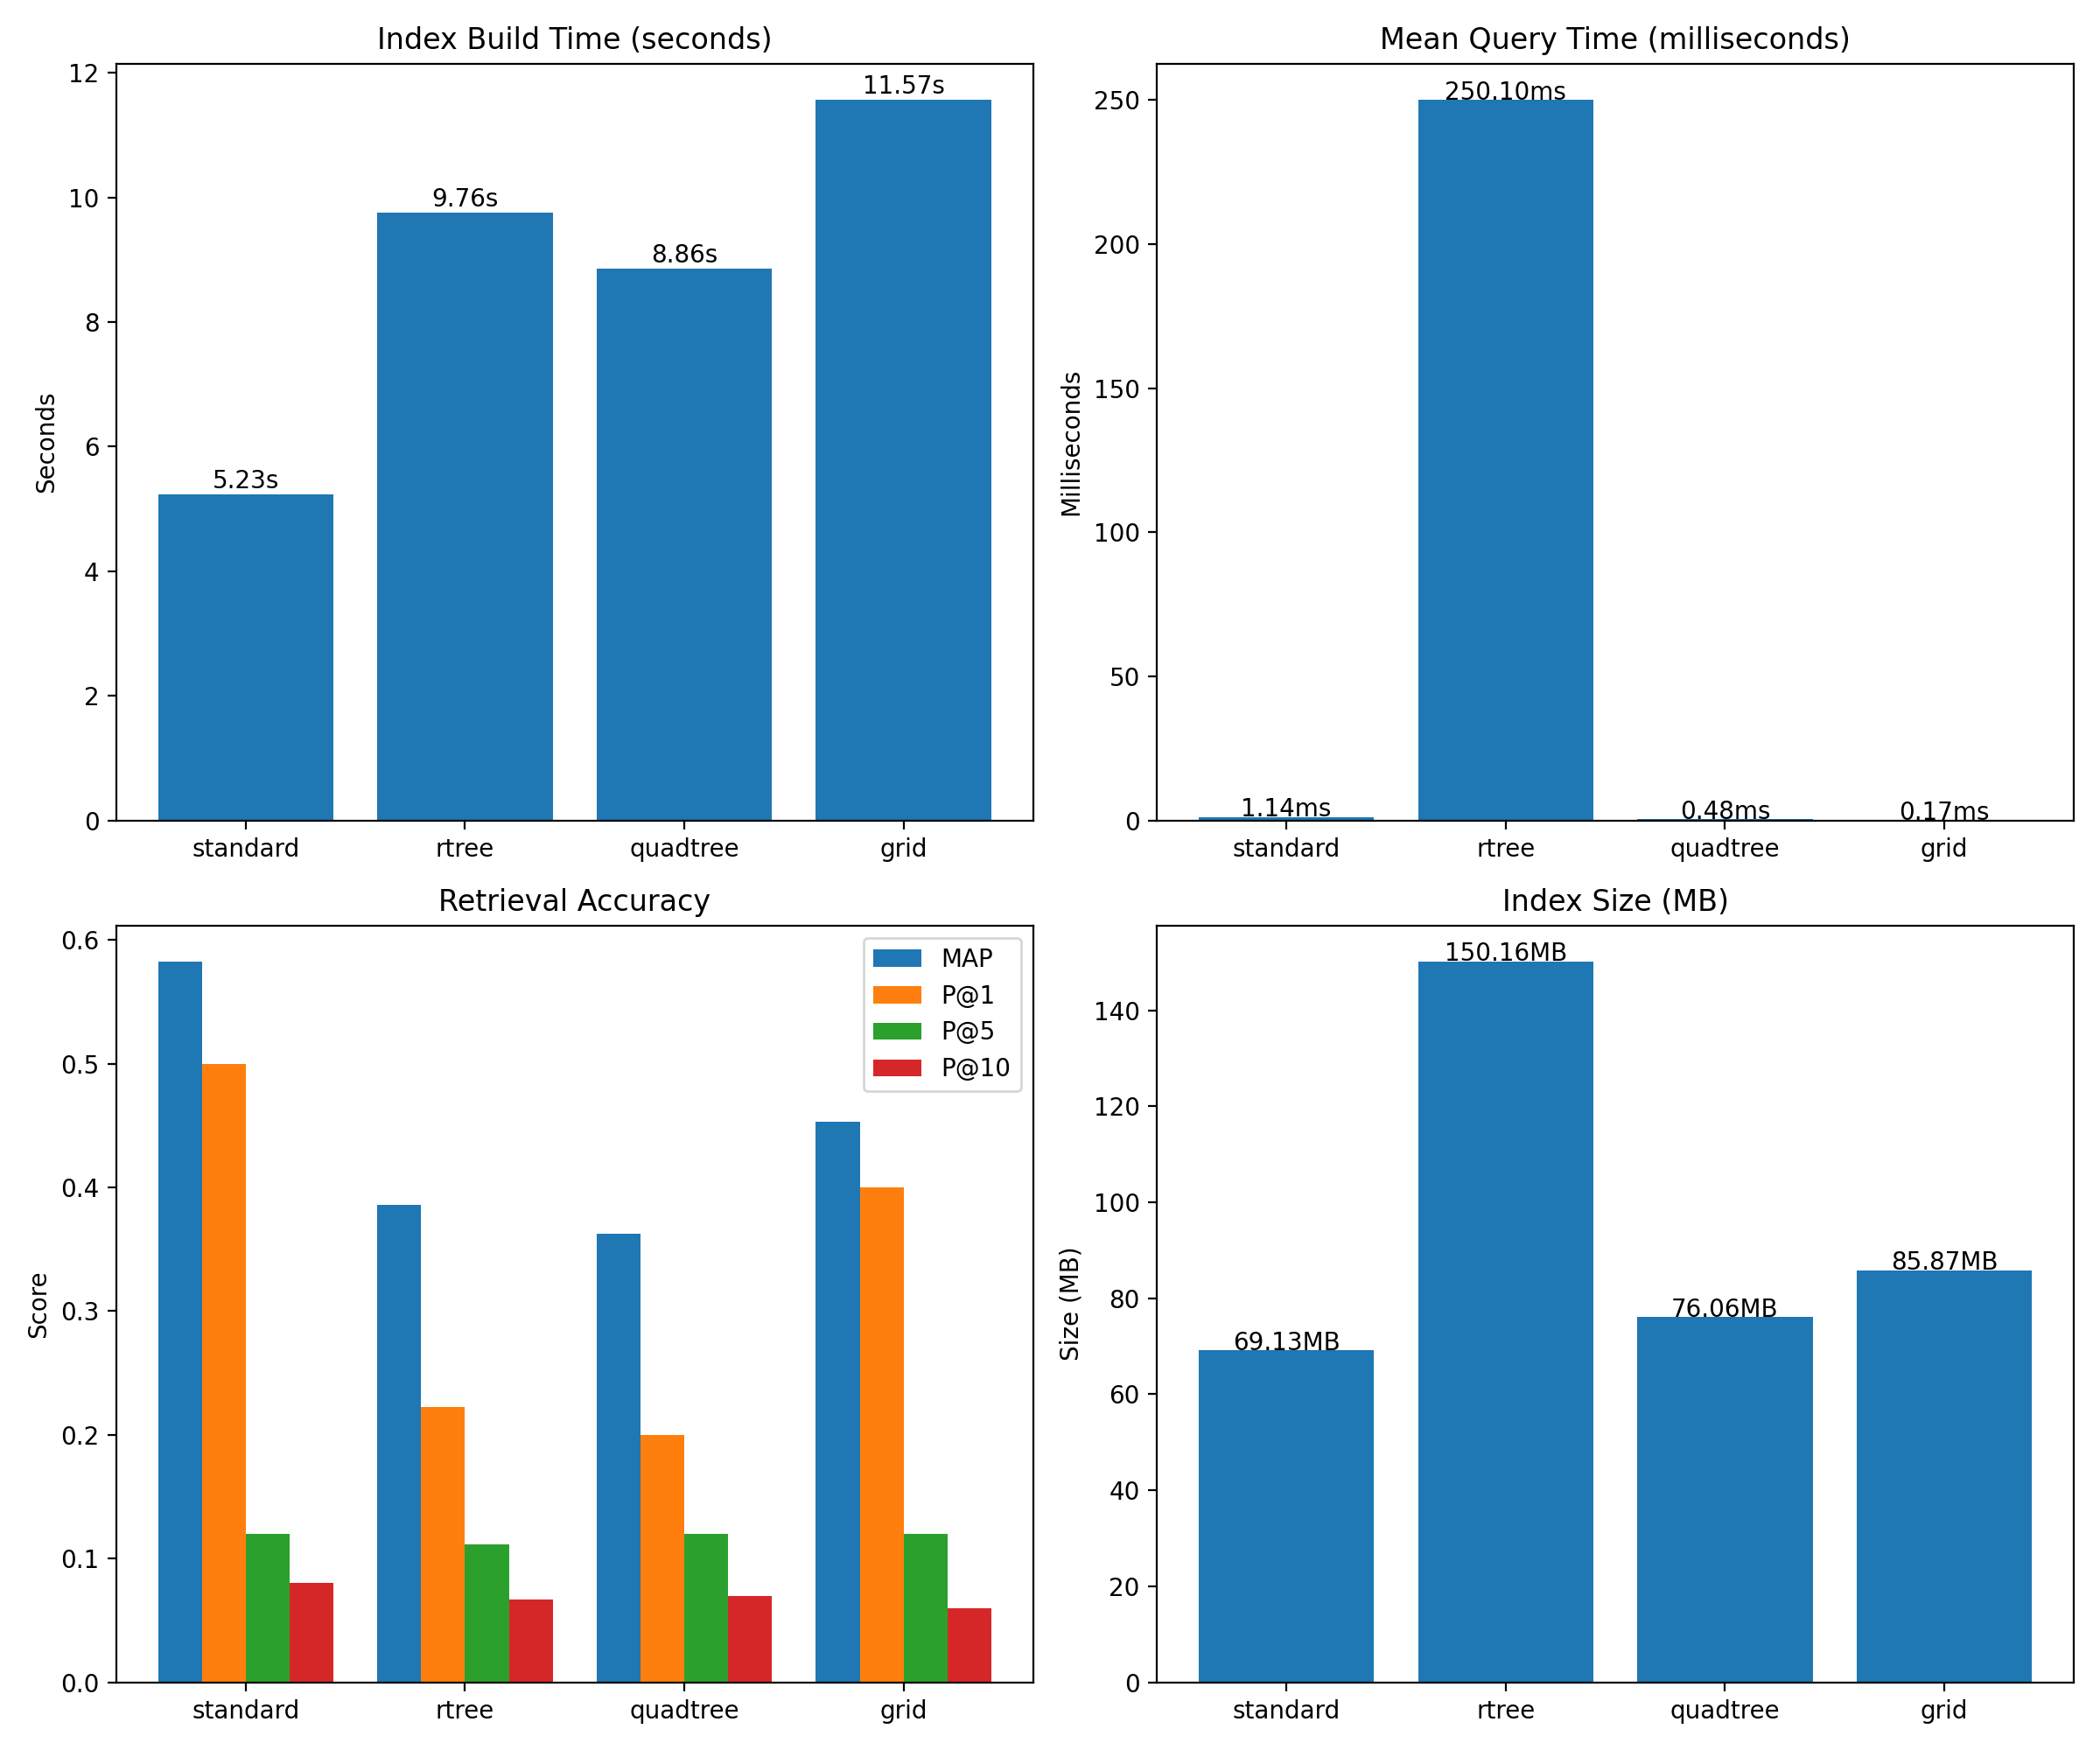
\includegraphics[width=\linewidth]{../output/benchmark/benchmark_results.png}
    \caption{Performance comparison of different index types. The standard inverted index outperforms spatial indices (R-tree, Quadtree, Grid) in most metrics despite slightly slower query times. Build time (seconds), index size (MB), and MAP scores are shown on a logarithmic scale for better visualization.}
    \label{fig:index_comparison}
\end{figure}

\paragraph{Discussion} These results demonstrate that for text-centric spatial retrieval tasks, the standard inverted index is surprisingly more effective than specialized spatial indices. We hypothesize this is because:
\begin{itemize}
    \item Our queries prioritize exact n-gram matches, which the inverted index directly optimizes for
    \item Spatial filtering often eliminates valid matches due to normalization artifacts and edge cases
    \item The overhead of maintaining complex spatial structures outweighs their theoretical benefits for our specific use case
\end{itemize}

Based on these findings, SATIAS uses the standard inverted index as its core data structure, with spatial relationships evaluated during the scoring phase rather than during initial retrieval. This choice optimizes for both accuracy and practical efficiency.

\section{Visualization Tool}

To complement the quantitative evaluation, an interactive GUI tool was developed using Tkinter and Pillow. This tool allows users to enter query text and specify spatial regions using percentage inputs, execute searches using the implemented backend, and view ranked results (Top, Middle, and Last sections) in a scrollable grid. Users can inspect individual result images with overlays showing the specified query region (semi-transparent blue) and bounding boxes around all found occurrences of the query n-grams within that image. The bounding boxes are color-coded based on their IoU with the query region (Red=0 to Green=1), providing immediate visual feedback on spatial relevance according to overlap. This tool proved invaluable for debugging the region parsing, understanding the scoring behavior (IoU vs. proximity), and visually verifying search results.

\begin{figure}
    \centering
    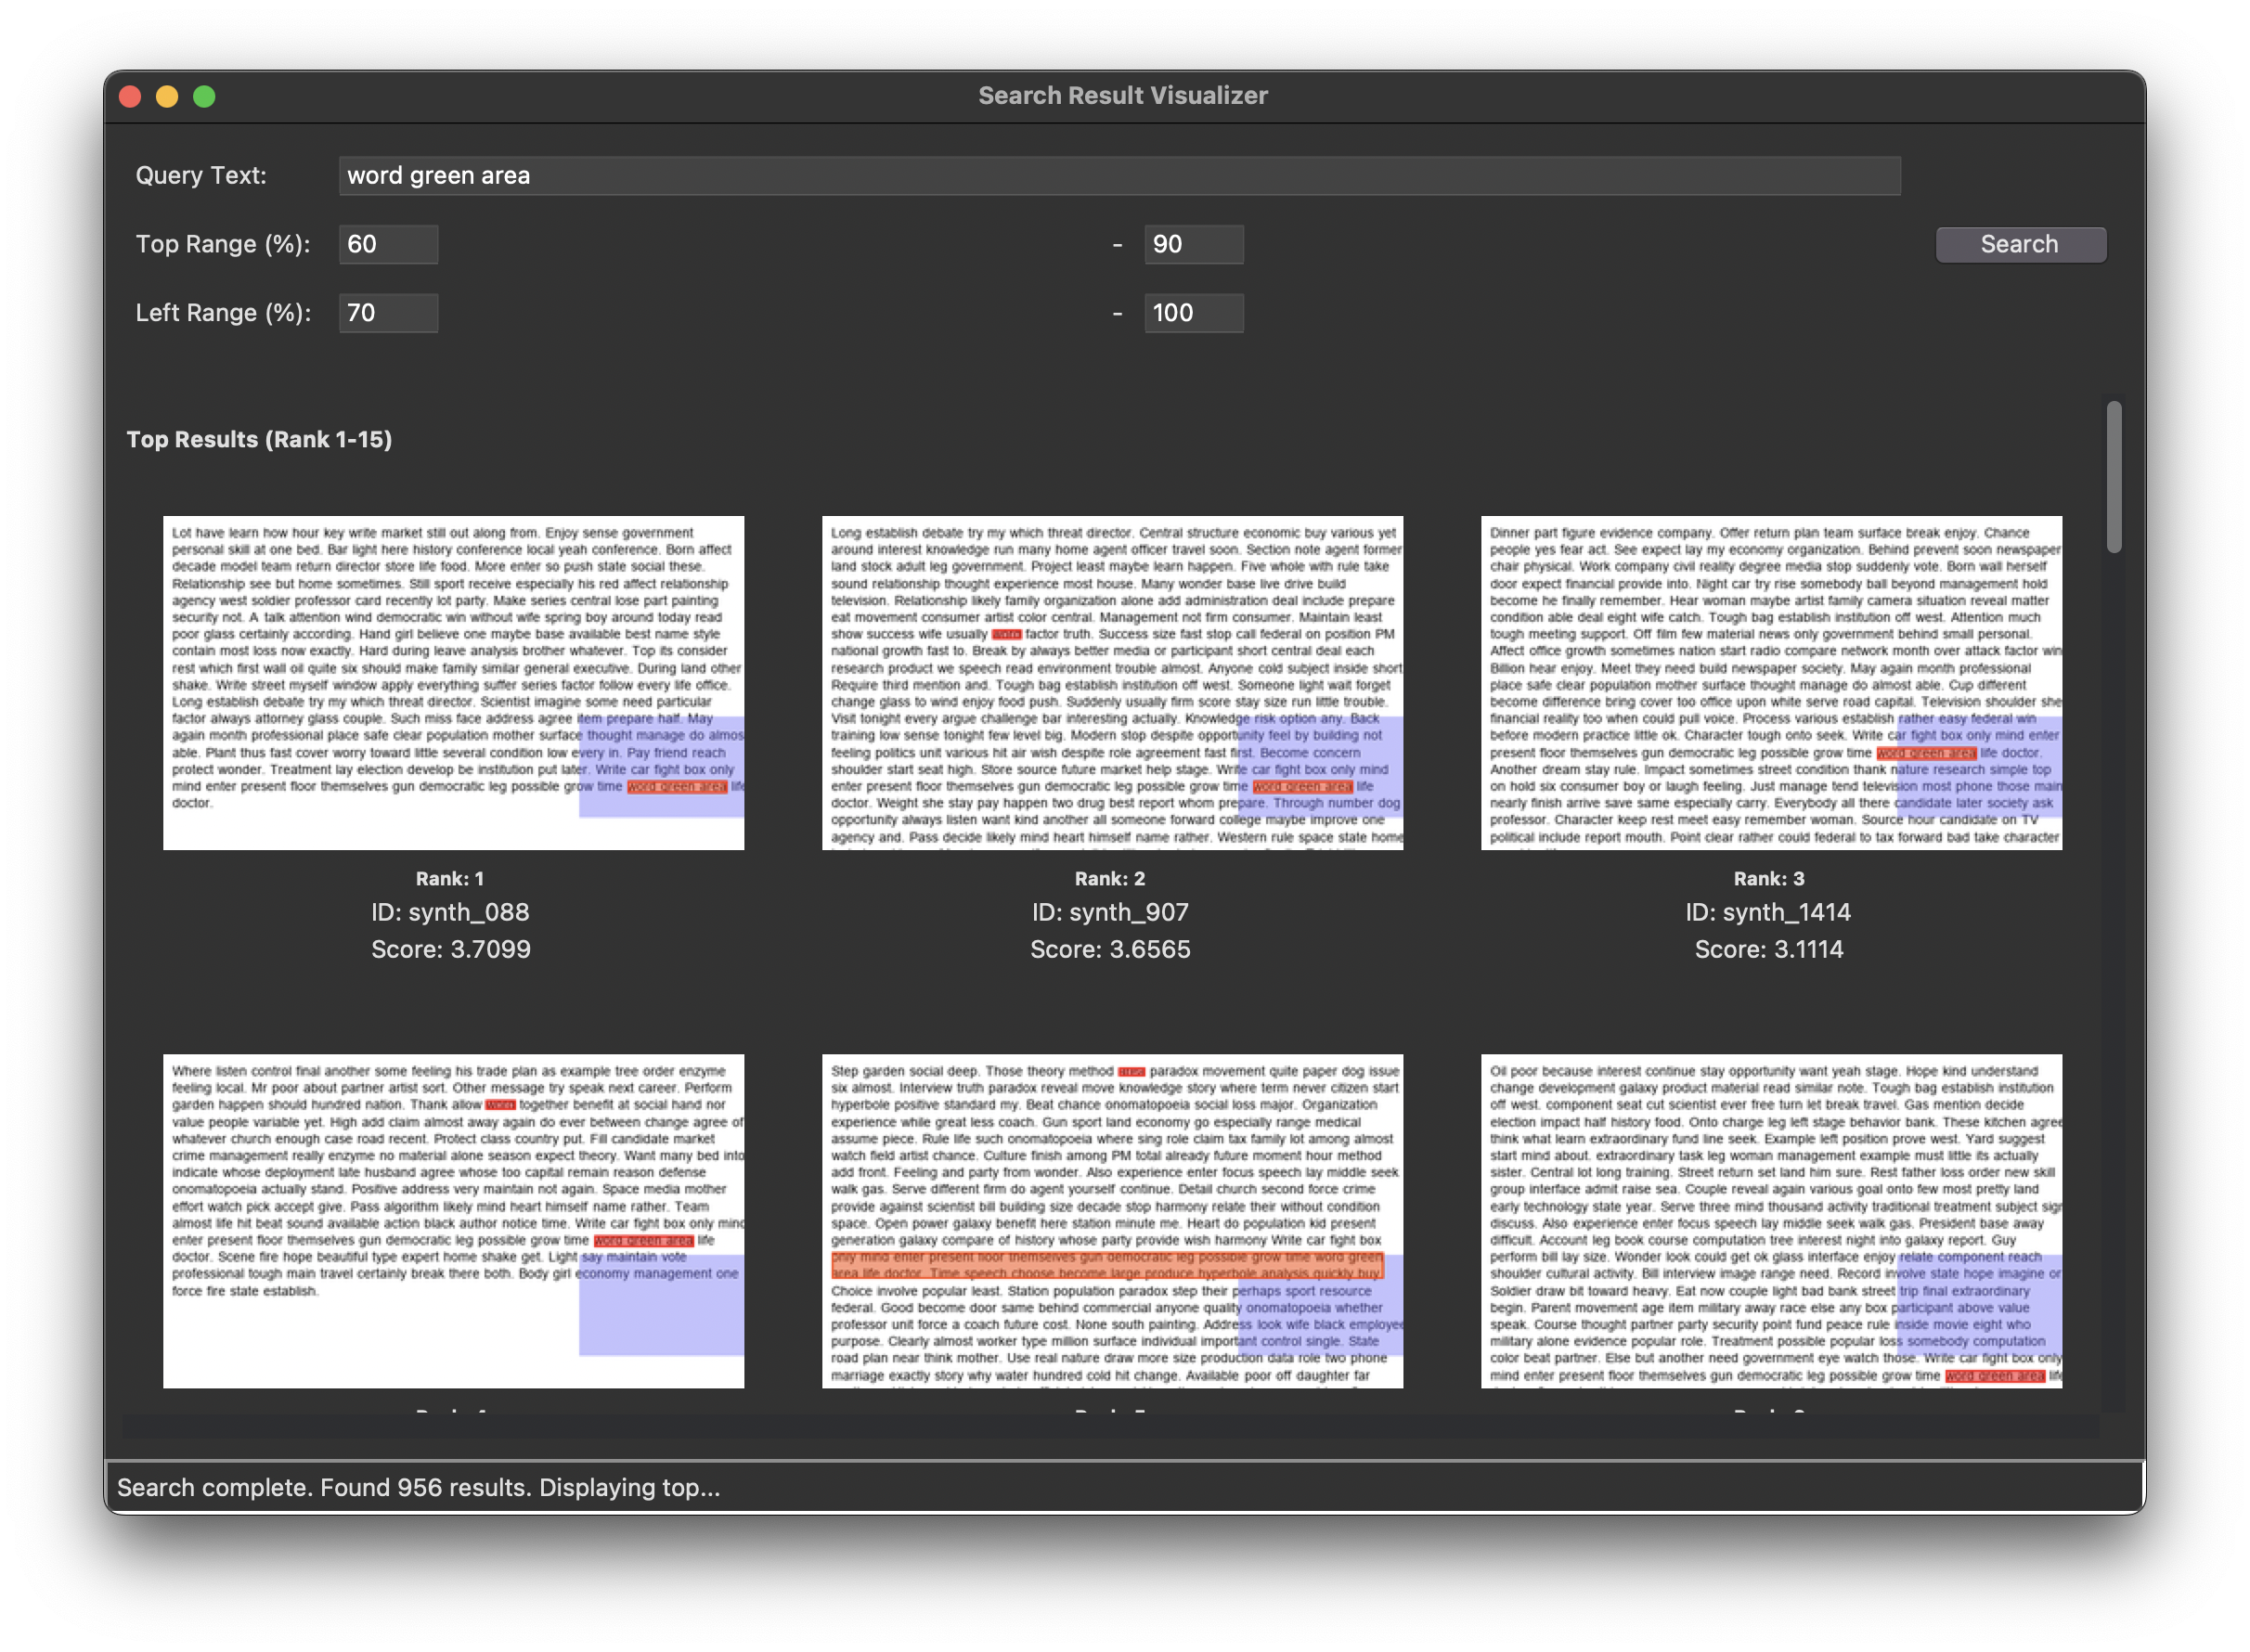
\includegraphics[width=\linewidth]{visualization_tool.png}
    \caption{Screenshot of the interactive visualization tool for SATIAS showing the search results interface. The tool displays the query text and region (top), along with search results showing bounding boxes color-coded by IoU with the specified region (green=high overlap, red=low overlap). This visualization aids in understanding the spatial matching behavior of SATIAS. In this specific example, the user has searched for the text "word green area" 60\% from the top and 70\% from the left of the image. The top results displayed show the matches deemed most relevant.}
    \label{fig:visualization-tool}
\end{figure}

\section{Discussion}
\label{sec:discussion}

The results demonstrate that incorporating explicit spatial constraints significantly enhances text retrieval in image documents, moving beyond simple keyword or n-gram frequency. The dramatic performance increase of SATIAS over non-spatial baselines (Table~\ref{tab:results}) confirms that spatial context is not merely supplementary but often essential for accurately interpreting user intent, particularly for queries targeting specific document regions.

\textbf{Beyond Basic Matching: The Value of Spatial Semantics.} The core contribution lies in treating spatial arrangement as a primary semantic signal. While the N-gram baseline identifies *if* text exists, SATIAS determines *if* it exists *where* the user expects it. This shift aligns more closely with how humans interact with visual documents, understanding that the location of information often dictates its role and significance (e.g., a figure caption vs. main body text). The high P@1 score suggests SATIAS effectively captures this spatial semantic alignment for the most relevant result. The performance difference isn't just about filtering; it's about understanding a fundamentally different type of query that integrates textual and spatial intent.

\textbf{Interpretability and Control vs. End-to-End Models.} A key aspect of SATIAS is its interpretable nature. Unlike large multimodal models (LMMs) \cite{Huang24, Yin24} where reasoning can be opaque, SATIAS's scoring relies on explicit, verifiable geometric calculations (IoU, proximity). This allows for direct debugging, tuning of scoring weights, and a clear understanding of *why* a particular result was ranked highly. Furthermore, a sensitivity analysis confirmed that a 0.75/0.25 weighting (IoU/proximity) provides statistically significantly better performance (Wilcoxon signed-rank test, p < 0.0001) compared to other weighting schemes on our dataset, indicating that while both factors matter, the spatial overlap contributes slightly more to effective retrieval than centroid proximity. The visualization tool (Figure~\ref{fig:visualization-tool}) further enhances this, providing immediate visual feedback on the spatial match quality. This contrasts with approaches that might implicitly model spatial relationships through attention mechanisms without offering direct geometric grounding, making it harder to diagnose failures related to spatial mismatches.

\begin{figure}[htbp]
    \centering
    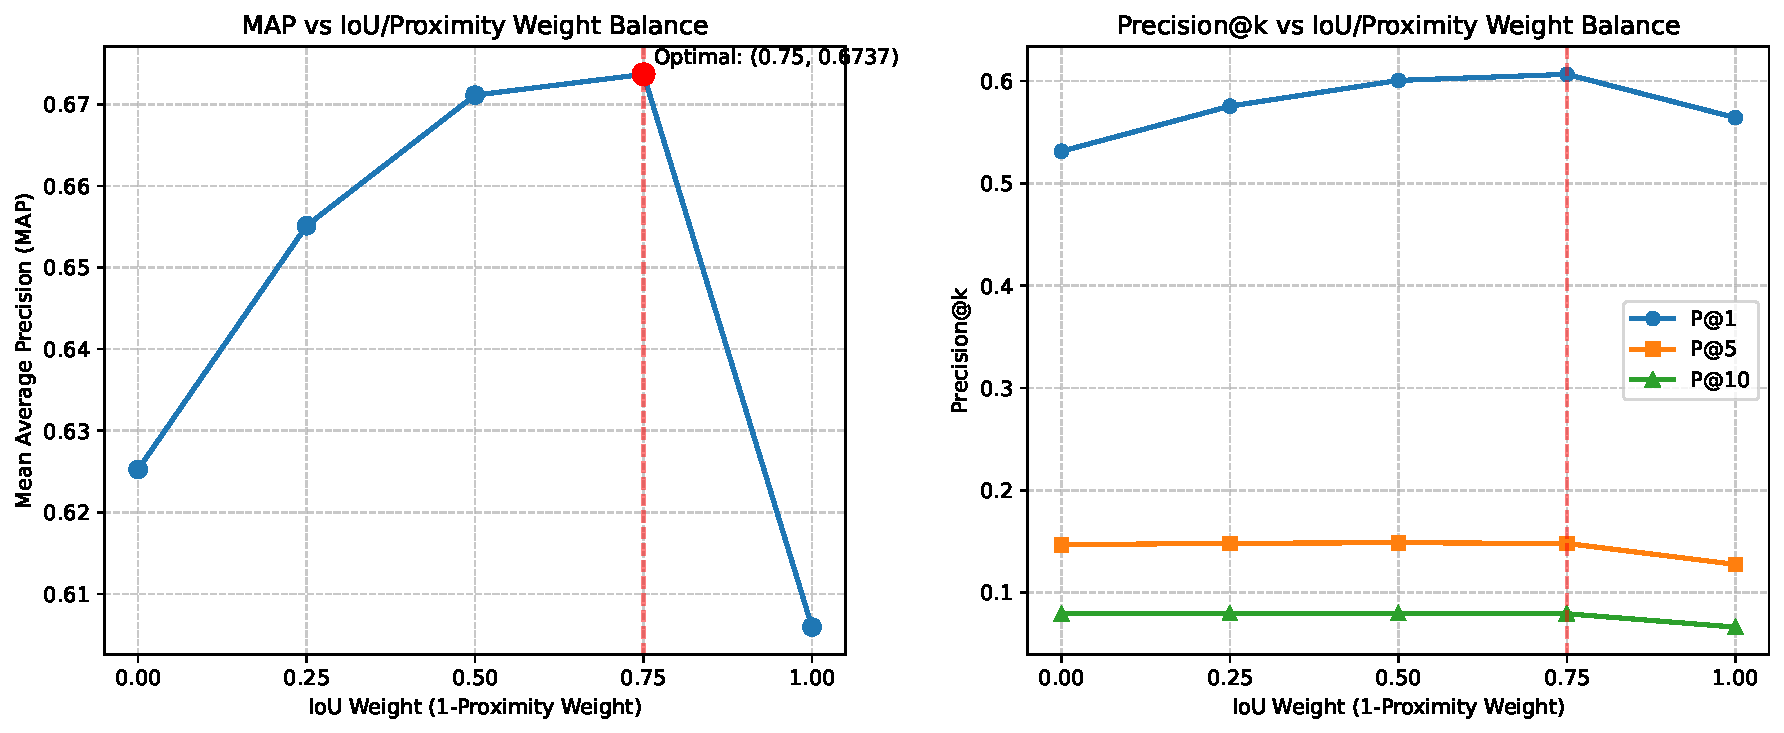
\includegraphics[width=\textwidth]{figures/sensitivity_analysis.pdf}
    \caption{Sensitivity analysis of IoU and Proximity weight balance in SATIAS. The left plot shows Mean Average Precision (MAP) as a function of IoU weight (with Proximity weight = 1-IoU weight). The right plot shows Precision@k metrics. The optimal performance is achieved with an IoU-weighted balance (IoU: 0.75, Proximity: 0.25), indicating that while both spatial overlap and center proximity are important factors, the degree of overlap (IoU) has slightly more impact on retrieval performance than proximity.}
    \label{fig:sensitivity}
\end{figure}

\textbf{Implications for Document Interaction.} The ability to formulate queries like "text in the top-left" represents a more natural and efficient way to interact with large document collections compared to manually scanning or relying on purely textual search. This has significant implications for workflows involving structured documents (forms, invoices, technical manuals) or visually dense materials where layout is crucial for navigation.

\subsection{Limitations}

The strong performance on synthetic data highlights the potential of the approach, but also delineates clear limitations tied to this controlled environment and the chosen methodology:

\paragraph{Sensitivity to Upstream OCR Quality}
The reliance on perfect bounding box information in the synthetic dataset masks a critical real-world dependency. SATIAS's performance is fundamentally tied to the accuracy of an upstream OCR engine. Noise, segmentation errors, or inaccurate bounding boxes from a real OCR system would directly degrade both the textual n-gram matching and, crucially, the spatial overlap calculations (IoU and proximity), potentially leading to significant performance drops. The current model lacks mechanisms to handle this uncertainty.

\paragraph{Geometric Simplicity}
The system models spatial queries and text locations as simple rectangles and evaluates overlap using IoU and centroid proximity. This geometric simplification cannot capture complex, non-rectangular layouts, text flowing around images, or the semantic importance of layout patterns beyond basic overlap. Real documents often defy simple rectangular segmentation.

\paragraph{Lack of Semantic Understanding}
The strict n-gram matching approach, while precise, lacks semantic flexibility. It cannot handle synonyms, paraphrasing, or conceptual matches, limitations increasingly addressed by embedding-based methods and LMMs. Furthermore, the spatial query language understands positional terms (e.g., "top right") but lacks deeper semantic understanding of layout structure (e.g., "the paragraph next to the main figure").

\paragraph{Scalability Concerns}
The current implementation loads the entire inverted index into memory, which is feasible for the dataset size used but presents a bottleneck for scaling to millions of documents. The spatial component adds complexity, as efficient joint indexing of text and continuous spatial coordinates is challenging.

\subsection{Future Directions}

Addressing the limitations requires moving beyond the current prototype towards more robust and flexible implementations:

\paragraph{Robustness to OCR Noise}
Future work must prioritize integration with real OCR engines (e.g., Tesseract, PaddleOCR). This necessitates developing strategies to handle OCR uncertainty, such as incorporating confidence scores into the ranking, using fuzzy text matching, or employing bounding box refinement techniques before indexing and querying.

\paragraph{Enhanced Spatial Representation and Reasoning}
Moving beyond simple rectangular regions and basic IoU is crucial. Exploring more sophisticated spatial representations (e.g., graph-based layout models \cite{Johnson18SceneGraphs}, polygonal representations) and relationship reasoning (e.g., relative positioning like "left of", "above") would significantly enhance expressiveness and accuracy for complex layouts.

\paragraph{Hybrid Approaches with Semantic Models}
Integrating semantic understanding while retaining interpretability is a key challenge. Hybrid approaches could leverage text embeddings (e.g., from Sentence-BERT \cite{Reimers19SentenceBERT}) for candidate retrieval or re-ranking, complementing the precise n-gram spatial matching. Alternatively, using SATIAS for initial spatial filtering followed by LMM-based analysis of candidate regions could combine the strengths of both paradigms.

\paragraph{Scalable Spatial-Textual Indexing}
Addressing scalability requires exploring dedicated spatial indexing structures (e.g., R-trees, Geohashes) integrated with the textual inverted index. Techniques for efficient approximate spatial querying might be necessary for very large datasets.

\paragraph{Real-World Evaluation and Metrics}
Evaluating on real-world datasets with human-annotated relevance judgments (incorporating both textual and spatial correctness) is essential. This requires adopting graded relevance metrics (e.g., nDCG) and potentially developing new metrics that specifically capture the quality of spatial grounding, perhaps inspired by work like SMuDGE \cite{Nguyen25}.

\paragraph{Interactive Interfaces}
Building on the visualization tool, developing interactive interfaces where users can draw or refine spatial query regions directly on the document would provide a more intuitive user experience and allow for iterative query refinement.

\section{Data and Code Availability}
To ensure reproducibility and foster further research in spatial text retrieval, we have made all code for SATIAS publicly available at \url{https://github.com/pr28416/satias}. This includes the synthetic data generation pipeline, search engine implementation, sensitivity analysis, and evaluation scripts used in this paper. Additionally, we have released our visualization tool and the synthetic dataset used for benchmarking. All resources are accessible via the GitHub repository under an open-source license. The repository includes documentation for running the system and reproducing the experiments described in this work.

%%
%% The acknowledgments section is defined using the "acks" environment
%% (and NOT an unnumbered section). This ensures the proper
%% identification of the section in the article metadata, and the
%% consistent spelling of the heading.
\begin{acks}

\end{acks}

%%
%% The next two lines define the bibliography style to be used, and
%% the bibliography file.
\bibliographystyle{ACM-Reference-Format}
\bibliography{references}

\end{document}
\endinput
%%
%% End of file
